\documentclass{article}

\usepackage[%
    left=0.5in,%
    right=0.5in,%
    top=0.5in,%
    bottom=0.5in,%
]{geometry}%
\usepackage{minitoc}
\usepackage{multicol}
\usepackage{graphicx}
\usepackage{fixltx2e}
\usepackage{listings}
\usepackage{color}
\usepackage{hyperref}
    \hypersetup{ colorlinks = true, linkcolor = blue }
\usepackage{blindtext}
\definecolor{lightgray}{gray}{0.9}
\graphicspath{ {./} }

\newcommand{\inlinecode}[2]{\colorbox{lightgray}{\lstinline
[language=#1]$#2$}}
\newcommand{\worddef}[1]{\hyperref[sec:reference]{\textit{#1}}}

\begin{document}

\tableofcontents

\newpage

\section{How can we save power for mobiles}

\begin{itemize}
  \item Knowledge about the power consumption of each component and app 
  \item Screen /network/CPU off or release other device resources as soon as not needed 
  \item Limit resources for less frequently used apps 
  \item Set device to sleep as soon as no user interactions 
  \item Global management of running jobs across all apps (i.e. perform syncs, upload/download together at fixed time window)
\end{itemize}

\subsection{Battery Consumption Statistics}

\begin{itemize}
  \item Framework tracks the time that devices spend in different states (e.g. WiFi chipset:on/off, Display :low/high brightness) 
  \item Controlling service pushes state changes to BatteryStats service. Framework pulls the data at these transition points 
  \item App consumption power is calculated based on CPU run time at specific speeds
\end{itemize}

\section{Android Power Management Concept}

\begin{itemize}
  \item  Designed for mobile devices 
  \item Goal is to prolong battery life 
  \item Based on Linux Power Management (\textbf{not suitable for a mobile device})
  \begin{itemize}
    \item – G0 (working) 
    \item – G1 (sleeping)
    \begin{itemize}
      \item S1 (CPU stops executing instructions, power to CPU and RAM maintained) 
      \item S2 (CPU powered off, cache is flushed) 
      \item S3 (Standby / sleep / suspend to powered RAM) 
      \item S4 (Hibernate / suspend to disk, RAM powered off) –
    \end{itemize}
    \item - G2 (S5, soft off) 
    \item – G3 (mechanical off) 
   \end{itemize}  
  \item Mobile phones have a default “off” behaviour
\end{itemize}

\subsection{Power Management Design}

\begin{multicols}{2}

\begin{itemize}
  \item A wrapper to Linux Power Management 
  \item Added to the Kernel – Wake Lock mechanism 
  \item Apps need to request CPU \& Screen to be on with WakeLocks, otherwise Android will shut down the CPU 
  \item Wake locks and timeouts constantly switch the state of the system’s power
  \begin{itemize}
    \item Overall system power consumption decreases
    \item “Better” use of battery capacity
  \end{itemize}
\end{itemize}

\vfill\null

\begin{center}
  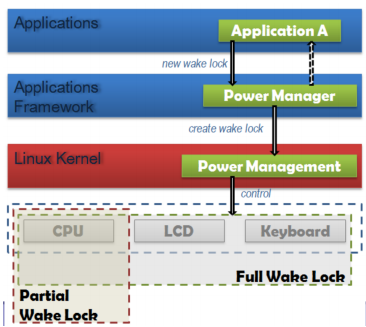
\includegraphics[scale=0.5]{power_architecture.png}
\end{center}

\end{multicols}

\section{Battery Life Enhancement in Android (Android 6.0 onwards)}

\begin{itemize}
  \item \textbf{App Standby}: defer background activity for apps with no recent user interaction. 
  \item \textbf{Doze}: deep sleep if user has not actively used the device for extended periods of time 
  \item \textbf{Exemptions}: system apps and cloud messaging services preloaded on phone are exempted from App Standby \& Doze. 
  \item Test apps in App standby \& Doze mode for the desired performance
\end{itemize}

\section{App Standby}

\begin{itemize}
  \item \textbf{Start conditions}: an app is not actively used for a certain time will be placed in an idle mode
  \begin{itemize}
    \item Not doing foreground work (activities/service, pending notifications)
    \item Hasn’t been explicitly launched for certain time (days). 
  \end{itemize}
  \item \textbf{Actions}: No network access, no background jobs, can set Alarms, can use wake locks, allow network access once per day 
  \item \textbf{Exists conditions}: plug in the device, do some foreground tasks
\end{itemize}

\subsection{App Standby Buckets (Android 9.0)}

\begin{flushleft}
Prioritize apps based on how recently and how frequently the apps are used
\begin{itemize}
  \item Active: currently or recently used 
  \item Working Set: regular use 
  \item Frequent: often used not everyday 
  \item Rare: not frequently 
  \item Never: never
\end{itemize}

\section{Doze}

\begin{itemize}
  \item \textbf{Starts Doze}: when device is in idle - screen off, on battery \& stationary. 
  \item \textbf{In Doze}: no network access; no CPU-intensive work; wakelocks ignored; no wifi scan; deferred alarm manager alarms; only high priority notification received; no job scheduler; no sync adapters. 
  \item \textbf{Exits Doze}: user interaction, device motion, screen on, or AlarmClock alarm. Notification do not cause Doze exits. 
  \item \textbf{Maintenance window}: complete pending activities (syncs, jobs, etc). • MMS/SMS/Telephony services are excluded from Doze
\end{itemize}

\section{Exemptions}

\begin{itemize}
  \item System apps and cloud messaging services preloaded on phone are exempted from App Standby \& Doze. 
  \item Use whitelist for apps to be partially exempt from Doze \& App Standby
  \begin{itemize}
    \item \verb|isIgnoringBatteryOptimiztions()| to check if in the whitelist;
    \item \verb|ACTION_IGNORE_BATTERY_OPTIMIZATION_SETTINGS| intent to direct user to battery optimization options 
    \item \verb|REQUEST_IGNORE_BATTERY_OPTIMIZATIONS| allow user to add app to whitelist directly 
  \end{itemize}
  \item Whitelisted apps can use network and hold partial wake locks during Doze \& App Standby, but jobs \& syncs are still deferred. 
  \item App should not be on the whitelist unless can’t use FCM high-priority messages or App’s core function is affected
\end{itemize}

\end{flushleft}

\section{Sustained Performance Mode (new API in Android 7.0)}
\begin{itemize}
  \item \textit{Thermal throttling prevents} a long running apps maintain its performance (e.g. game, camera, virtual reality application etc.) 
  \item App can request the platform to enter a SPM, and keep a consistent level of performance
  \begin{itemize}
    \item Only tests on Android 7.0 on Nexus 6P devices 
    \item Set using \verb|Window.setSustainedPerformanceMode()|
    \item System automatically disables the mode when no longer in focus
  \end{itemize}
\end{itemize}

\section{Schedule Jobs in Android}

\begin{flushleft}
For any timing operations that occur only during the lifetime of your application, it is best to use \textbf{application resources} (i.e. handler class) rather than system resources (e.g. Alarm manager/job Scheduler) to schedule tasks.
\end{flushleft}
\begin{itemize}  
  \item AlarmManager ($ < $ API 21) – Based on time. Only use when need to execute for specifc time.
  \item JobScheduler ($ \geq $API 21) – Based on conditions 
  \item Firebase Job Dispatcher ($ > $API 14) – Similar to JobScheduler but can be used for lower APIs and requires GooglePlay service 
  \item Work Manager (New) – Requires GooglePlay service – Automatic use of alarmManager and jobScheduler
\end{itemize}

\subsection{AlarmManager}

\begin{itemize}
  \item Schedule a task run at a specific time point/ time interval 
  \item AlarmManager holds a CPU wake lock, when alarm receiver’s onReceive() is executing 
  \item Alarm delivery is inexact (Android 5.0+); use setWindow and setExact for exact delivery.
\end{itemize}

\subsubsection{AlarmManager Usage}

\begin{itemize}
  \item Specify an Intent to be broadcast at some time
  \begin{itemize}
    \item setRepeating(int type, long triggerAtMillis, long intervalMillis, PendingIntent operation)
    \item setExact(int type, long triggerAtMillis, PendingIntent operation)
  \end{itemize}
  \item Extend Broadcast Receiver
  \begin{itemize}
    \item onReceive method is called when the alarm goes off
    \item Start a service to actually do the work
  \end{itemize}
\end{itemize}

\subsection{Efficient Scheduling}

\begin{itemize}
  \item Multiple scheduled alarms waking the phone: Suspending and waking the phone takes power 
  \item More efficient to schedule multiple alarms at the same time
\end{itemize}

\subsection{JobScheduler}

\begin{itemize}
  \item Many apps perform tasks asynchronously outside the main activity. (e.g download files, sync database to cloud etc.) 
  \item Job Scheduler collects pending jobs across all apps, and schedule them to \textbf{run at about the same time}-> sleep for longer-> save power 
  \item Specify requirements for network and timing for each job, then the JS robustly optimise the execution time. 
  \item May defer jobs that comply with Doze & App Standby 
  \item JobService will run on the main thread. Need to manage any asynchronous tasks yourself (e.g. Threads).
\end{itemize}

\pagebreak
\section*{Reference section} \label{sec:reference}
\begin{description}
	\item[placeholder] \hfill \\
\end{description}
\end{document}
